
%
\documentclass[12pt,oneside,letterpaper]{report}
\usepackage[spanish]{babel}
\usepackage[ansinew]{inputenc}
\usepackage{graphicx}
\usepackage[right=2cm,left=3cm,top=2cm,bottom=2cm,headsep=0cm,footskip=0.5cm]{geometry}

%-------------------------------------------------------------------------
%definici�n de comandos

\newcommand{\dotrule}[1]{\parbox[t]{#1}{\dotfill}}

%para c�digo fuente
\newenvironment{codigoenv}
{\fontsize{10pt}{12pt} \linespread{1}} { \normalsize}

%para las imagenes
\newenvironment{figuraenv}
{\begin{figure}[htb]\begin{center}} {\end{center}\end{figure}}


\newcommand{\df}[2]{\textit{#1 (#2)}} %definicion de termino y sigla
\newcommand{\cls}[1]{\mbox{\textit{#1}}} %nombre de clase o paquete o c�digo
\newcommand{\trm}[1]{\textit{#1}} %termino tecnico o en ingles
\newcommand{\cod}[1]{\texttt{\footnotesize #1}} %codigo fuente

%-------------------------------------------------------------------------


\linespread{1}
\setlength{\parskip}{1\baselineskip}
\parindent 1cm
\sloppy


%-------------------------------------------------------------------------

\begin{document}

%-------------------------------------------------------------------------
\thispagestyle{empty}
\begin{center}

UNIVERSIDAD DE CHILE\\
FACULTAD DE CIENCIAS F�SICAS Y MATEM�TICAS\\
DEPARTAMENTO DE CIENCIAS DE LA COMPUTACI�N\\

\vspace{4cm}

CC4102 - Dise�o y Analisis de Algoritmos

\vspace{3cm}

Tarea 3: Busqueda



\vspace{9cm}
\begin{flushright}
\begin{tabular}{l}
Cristian Carre�o Medina\\
Diego Ch�vez Escobar\\
Prof. Jeremy Barbay; Aux. Mauricio Quezada
\end{tabular}
\end{flushright}
\vfill


\end{center}

%-------------------------------------------------------------------------

%-------------------------------------------------------------------------

%-------------------------------------------------------------------------
\newpage \pagenumbering{roman}
\tableofcontents

%-------------------------------------------------------------------------


%-------------------------------------------------------------------------
\newpage
\pagenumbering{arabic}
\chapter{Presentaci�n}

\section{Introducci�n}

El objetivo de este informe es comparar 3 algoritmos de b�squeda en 4 contextos distintos: elementos
con distribuci�n uniforme/no uniforme, y b�squedas con distribuci�n uniforme/no uniforme. 

Los 3 algoritmos a estudiar son los siguientes

\begin{enumerate}
\vspace{1cm}
\item
Busqueda Binaria
\item
Busqueda por Interpolacion
\item
Busqueda Inter-Mixta
\end{enumerate}


%-------------------------------------------------------------------------
\newpage
\chapter{Hipotesis}

\section{Dise�o Experimental}

Se desarrollara funciones que creen las variables de instacias uniformes y no uniformes, ademas de las variables de busquedas asociadas al dominio.
Luego se ejecutaran con los diversos algoritmos de busquedas en estudio, determinado el tiempo estadistico (por lo cual se requerira varias ejecuciones), las comparaciones totales y unitarias.
Este experimento se repetira para diversos valores de N correspondiente al arreglo de instancias.
Ademas se considera un arreglo M, que es el arreglo de busqueda, para caso experimentales estos seran arreglos de busqueda mas grandes que los arreglos de instancia, $4x$ y $8x$ mas grandes que el arreglo de instancia en ejecucion.

\subsection{Algoritmos de busqueda}

\subsubsection{Busqueda Binaria}

Busqueda que en cada etapa hace una comparaci�n
entre los dos elementos considerados, y hace una comparaci�n solamente cuando el rango
de inserci�n del elemento x es definido.


\subsubsection{Busqueda por Interpolacion}

Busqueda que usa el valor de x, y los valores a los extremos $(i < j)$ del
subarreglo actual, para interpolar la pr�xima posicion $g = i + (j - i)/(x - A[i])$ a comparar con x.


\subsubsection{Busqueda Inter-Mixta}

Busqueda que alterna los pasos de una b�squeda binaria con los pasos de una
b�squeda por interpolaci�n.


\section{Hipotesis}

Como hipotesis se espera que al efectuase sobre un arreglo distribuido sea la busqueda por interpolacion que posea mejores tiempos de ejecucion versus la busqueda binaria.

Ademas se espera que independiente de la las variables de instacia y busqueda, la busqueda binaria no se vea afectada por la variacion de estas variables.

Se espera que la busqueda binaria posee comparaciones unitarias contantes, debido a la estructura propia de una busqueda binaria.

Ademas se espera que la busqueda Inter-Mixta obtenga resultados entre ambas busquedas, demostrando que obtiene tiempos de ambos algoritmos.

%-------------------------------------------------------------------------

\newpage

\chapter{Resultados}


En las siguientes tablas se detallaran los resultados obtenidos para los 3 algoritmos de busqueda, se entregan resultados incluyendo tiempos estadisticos, comparaciones totales y unitarias.

A modo de simplificacion se usaran abreviaciones para el resto del presente informe estas abreviaciones son para las variables de instancia y busqueda: Aleatoria-Uniforme (A-U), Aleatoria-Inicio (A-I), Aleatoria-Dominio (A-D).

Ademas como dato el equipo utilizado para la experimentacion corresponde a un equipo portatil con disco
duro de 5400 rpm, 4 gb de ram, procesador Intel I7 2,2 ghz, Sistema operativo Ubuntu
12.04 de 64 bits y el lenguaje utilizado fue python.


%-------------------------------------------------------------------------




\begin{figure}
\section{Busqueda Binaria}
  \centering
    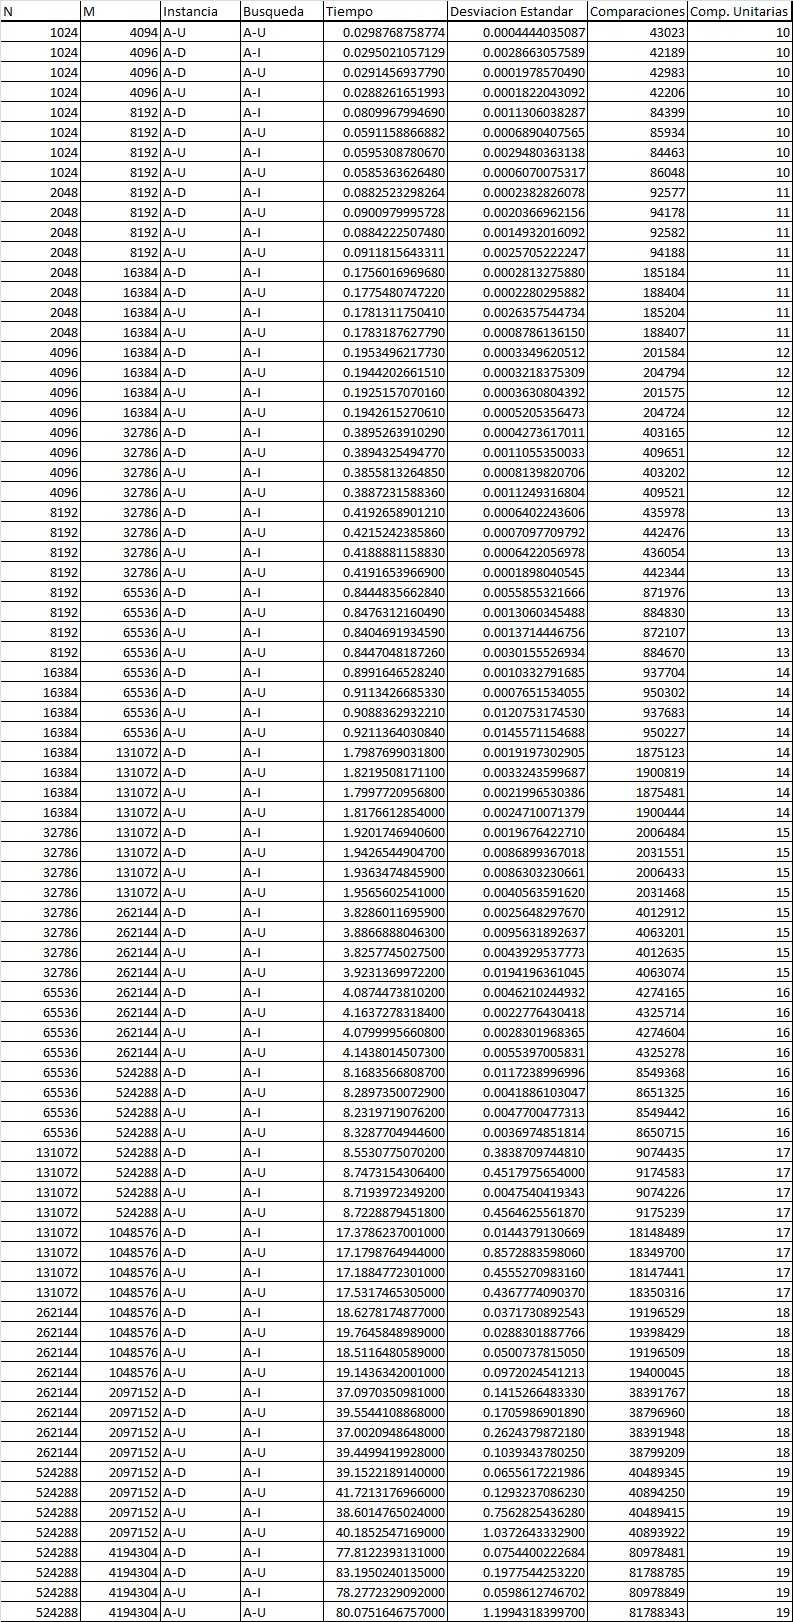
\includegraphics[width=0.65\textwidth]{ResultadosBinaria}
  \caption{Resultados Busqueda Binaria}
  \label{fig:BB}
\end{figure}



\begin{figure}
\section{Busqueda por Interpolacion}
  \centering
    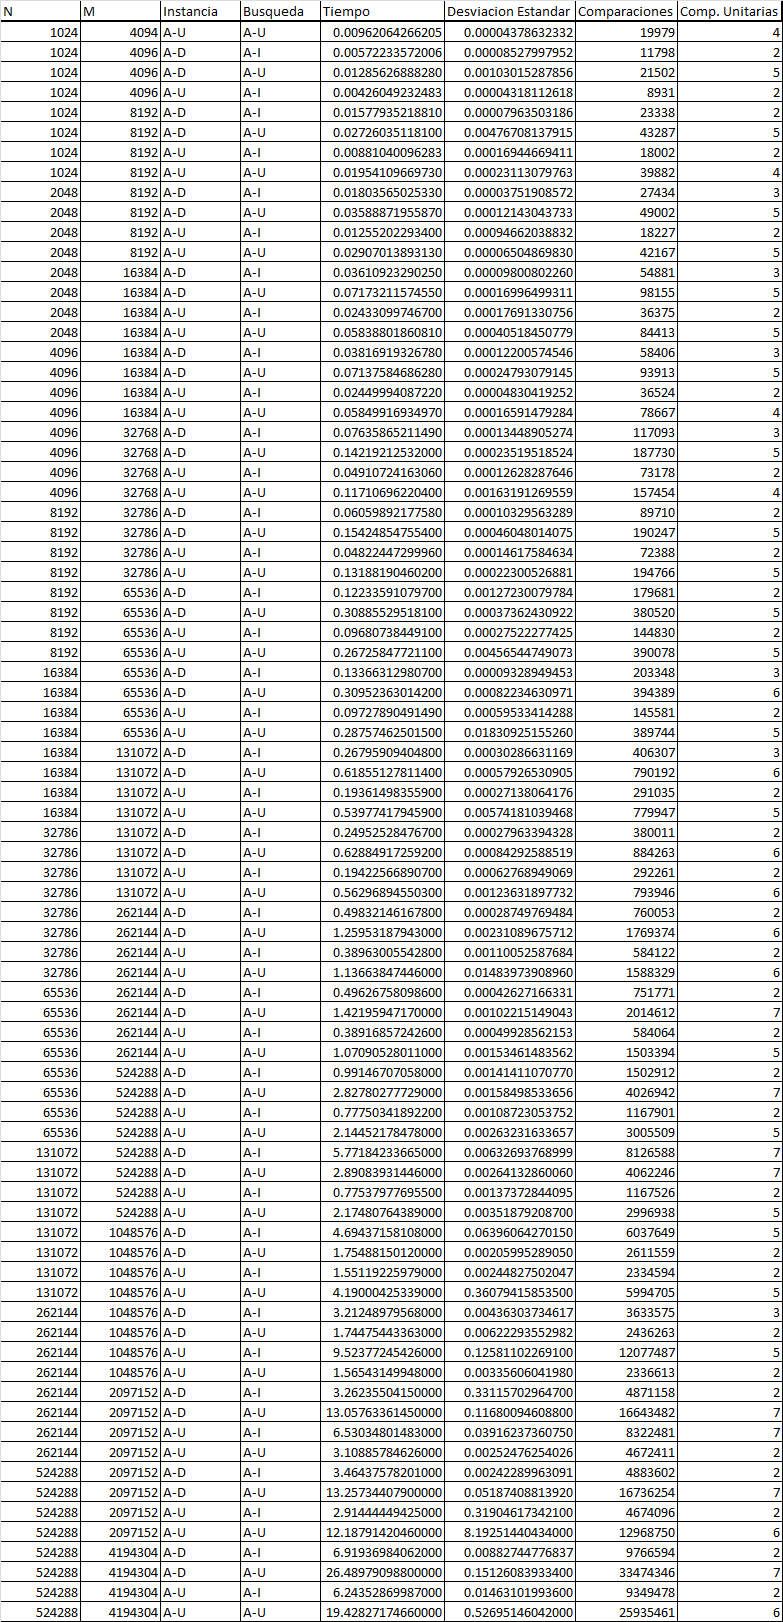
\includegraphics[width=0.64\textwidth]{BusquedaInterpolacion}
  \caption{Resultados Busqueda Por Interpolacion}
  \label{fig:BB}
\end{figure}



\begin{figure}
\section{Busqueda Inter-Mixta}
  \centering
    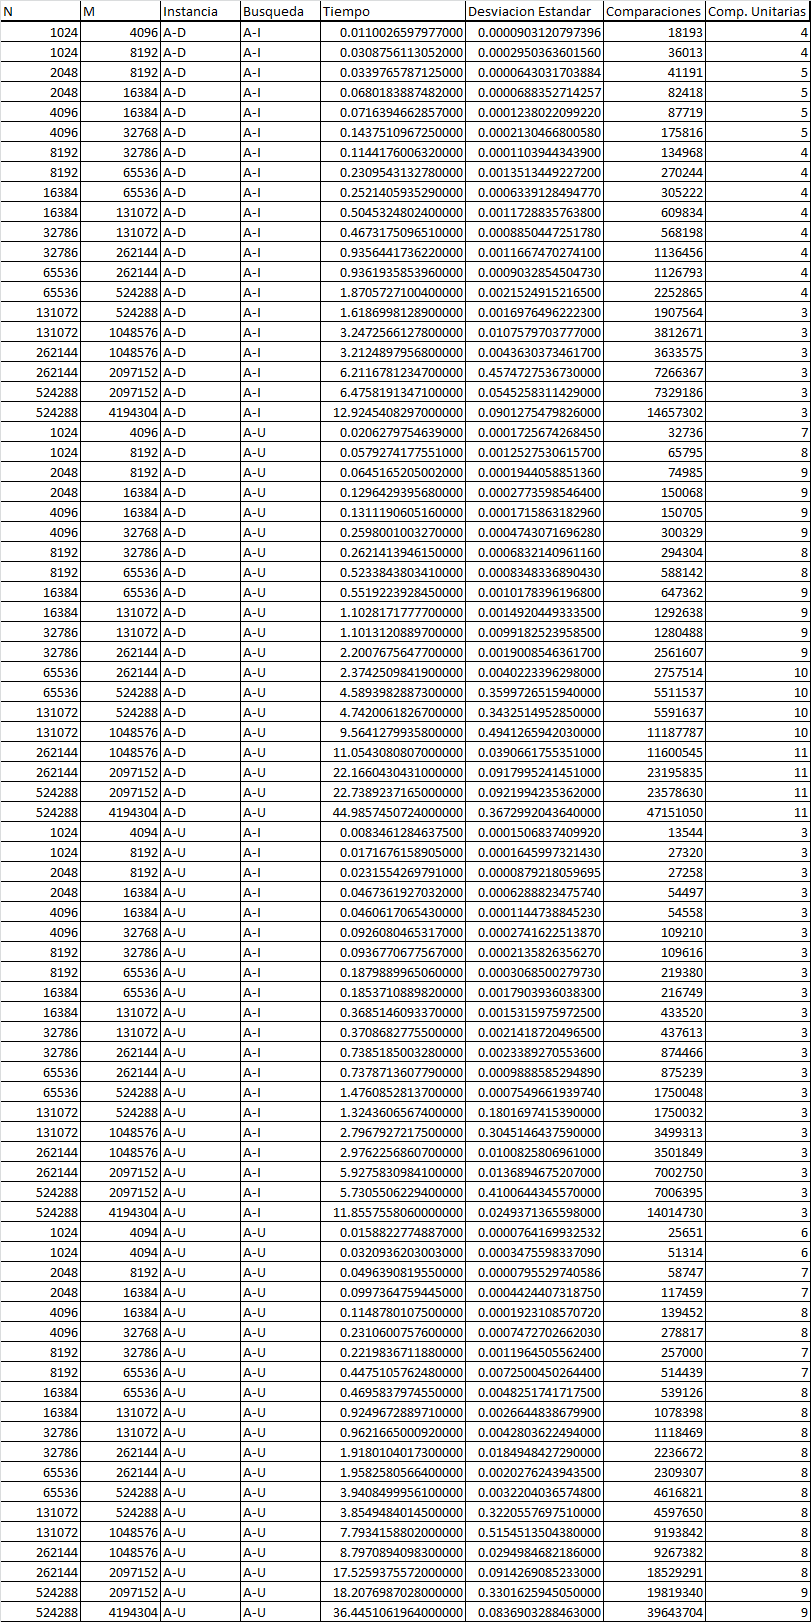
\includegraphics[width=0.65\textwidth]{ResultadosInter-Mixta}
  \caption{Resultados Busqueda Inter-Mixta}
  \label{fig:BB}
\end{figure}




%-------------------------------------------------------------------------
\newpage
\chapter{Analisis}



\section{Graficos}

Se adjuntaran solo los graficos que entreguen alguna conclusion grafica importante para el estudio y el desarrollo de posteriores conclusiones.

Los graficos presentados compara los resultados de tiempo y numero de comparaciones para los 3 algoritmos de busqueda estudiados, estos graficos muestra los resultados dependiendo de la variables de instacia y busqueda de cada experimento.

Ademas se entregan graficos que muestra comparacion de tiempos de ejecucion para el mismo algoritmo segun las variables de instacia y busqueda.

Estos graficos se anexaran al final del capitulo.




\section{Interpretacion de Resultados}



Como se esperaba la busqueda por interpolacion presento mejores resultados de tiempo de ejecucion y comparaciones, ya que si bien en arreglos de datos peque�os los tiempos se mantienen similares para ambos algoritmos es la busqueda binaria que se dispara al realizar en arreglos de datos grandes.

Ademas como era de esperar la busqueda Inter-Mixta entrega buenos resultados en arreglos peque�os pero al realizarse en arreglos grandes dispara sus tiempo de ejecucion debido a los pasos de busqueda binaria que realiza.

Los analisis anteriores aplican para las diversas combinaciones de variables de instancia y busqueda estudiadas.

El otro dato que salta a la vista de los analisis de datos es que la busqueda binaria posee comparaciones unitarias constantes solo dependientes del tama�o de N, esto afirma lo propuesto en la hipotesis. Ademas la busqueda binaria posee tiempos de ejecucion similares independientes de las variables de instancia y busqueda, es decir su ejecucion es contante independiente del caso.

Respecto a la busqueda por Interpolacion e Inter-Mixta, posee menores tiempos de ejecucion cuando las variables de busqueda se encuentran Aleatorias-Inicio(AI), ademas si las variables de instancia son Aletorias-Uniformes(AU) esta busqueda poseen mejores resultados aun.

Sobre la diferencia que puede determinar un arreglo de busqueda mayor al de instancia se puede determinar que entre mayor sea el arreglo de busqueda mayor seran los tiempos de ejecucion, esto independiente del algoritmo a estudiar.

\newpage
\begin{figure}
\newpage
  \centering
    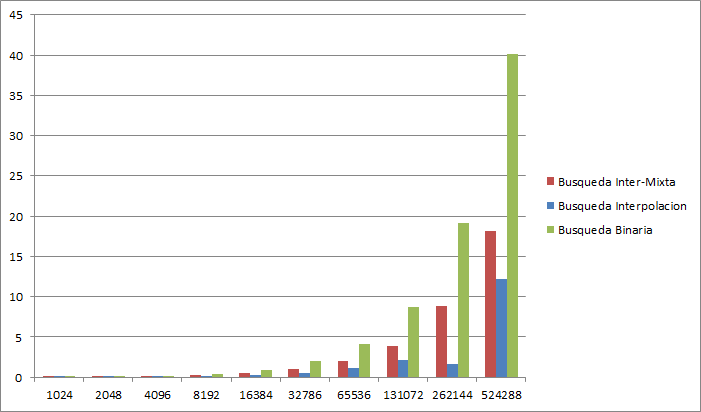
\includegraphics[width=0.9\textwidth]{tiempovsn,AU-AU}
  \caption{Tiempos AU-AU}
 
  \centering

    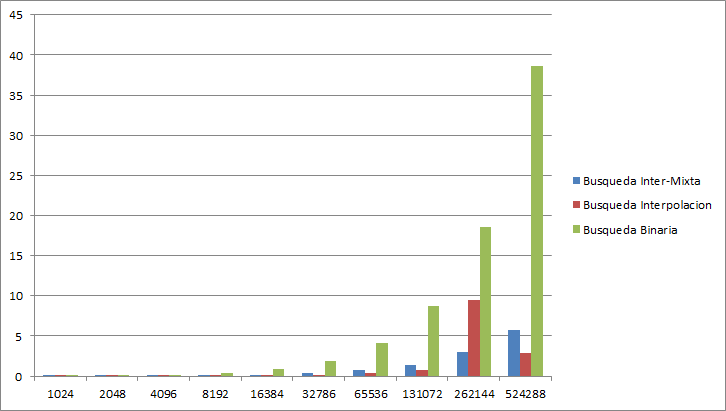
\includegraphics[width=0.9\textwidth]{tiempovsn,AU-AI}
  \caption{Tiempos AU-AI}
 
\end{figure}
\begin{figure} 
  \centering
    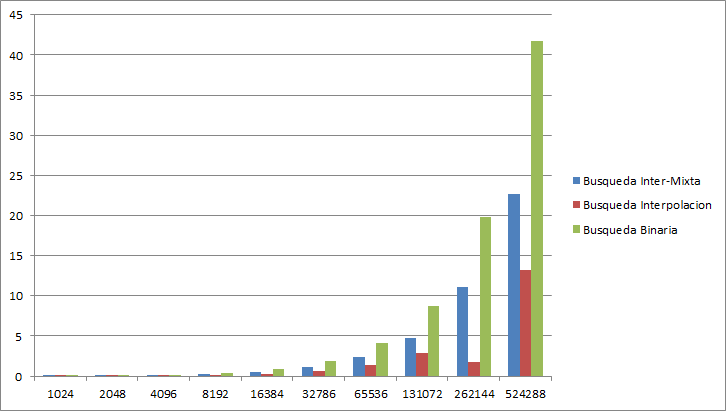
\includegraphics[width=0.9\textwidth]{tiempovsn,AD-AU}
  \caption{Tiempos AD-AU}
   
  \centering
 
    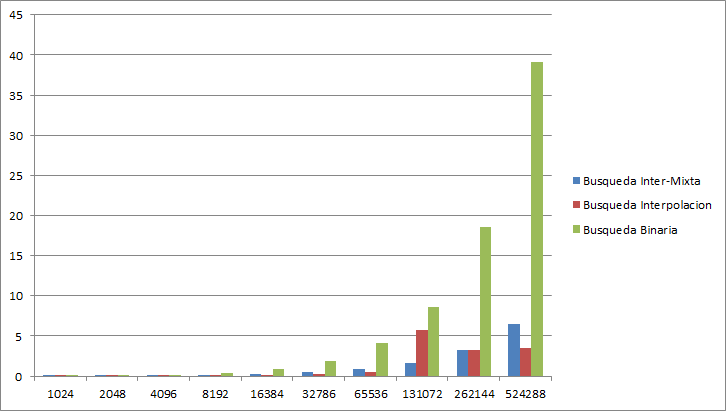
\includegraphics[width=0.9\textwidth]{tiempovsn,AD-AI}
  \caption{Tiempos AD-AI}
\end{figure}

\begin{figure}
  \centering
    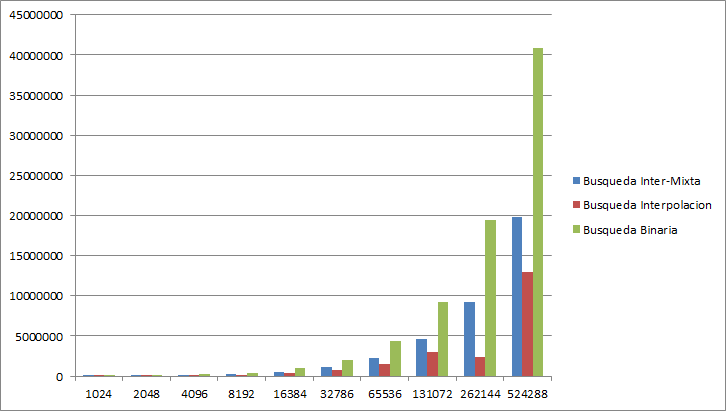
\includegraphics[width=0.9\textwidth]{Comparacionesvsn,AU-AU}
  \caption{Comparaciones AU-AU}
 
  \centering

    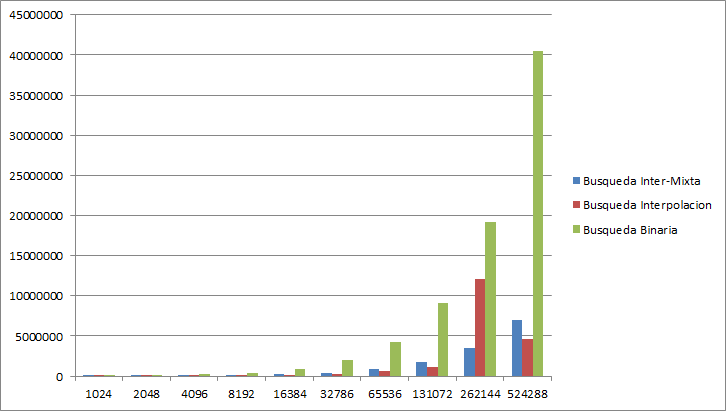
\includegraphics[width=0.9\textwidth]{Comparacionesvsn,AU-AI}
  \caption{Comparaciones AU-AI}
 
\end{figure}

\begin{figure} 
  \centering
    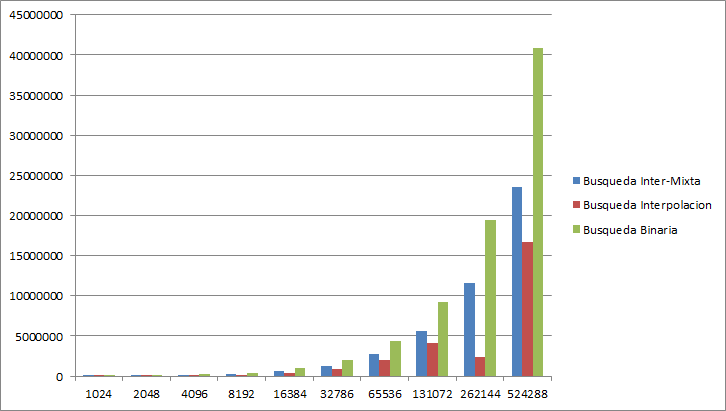
\includegraphics[width=0.9\textwidth]{Comparacionesvsn,AD-AU}
  \caption{Comparaciones AD-AU}
   
  \centering
 
    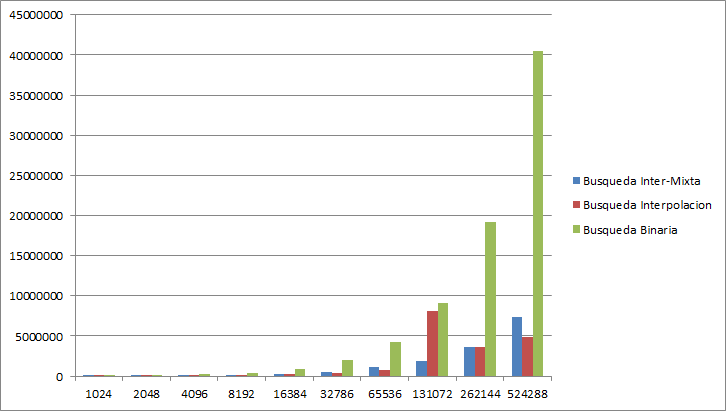
\includegraphics[width=0.9\textwidth]{Comparacionesvsn,AD-AI}
  \caption{Comparaciones AD-AI}
\end{figure}

\begin{figure} 
  \centering
    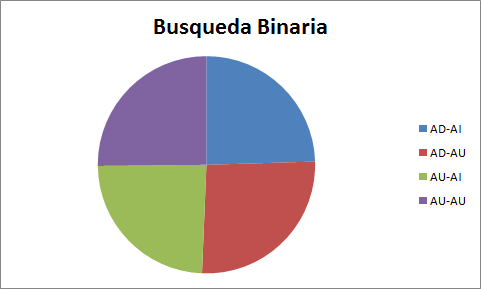
\includegraphics[width=0.65\textwidth]{BBinariaA-A}
  \caption{Resultados busqueda binaria, segun instancia busqueda}
   
  \centering
 
    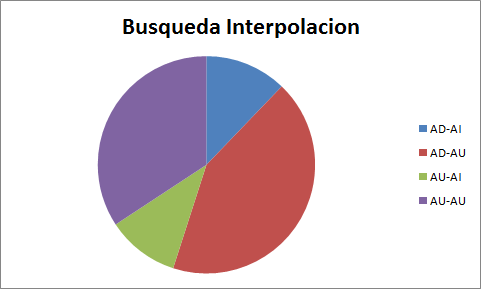
\includegraphics[width=0.65\textwidth]{BInterpolacionA-A}
  \caption{Resultados busqueda por interpolacion, segun instancia busqueda}
  
  \centering
 
    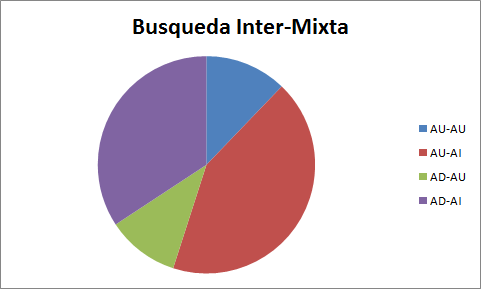
\includegraphics[width=0.65\textwidth]{BInter-MixtaA-A}
  \caption{Resultados busqueda inter-mixta, segun instancia busqueda}
  
\end{figure}

%-------------------------------------------------------------------------


%-------------------------------------------------------------------------
\newpage
\chapter{Conclusiones}
\section{Conclusiones}


Del presente informe se puede concluir que la para arreglos de datos grandes, donde se tiene una distribucion ya sea uniforme o no uniforme esta busqueda se puede ser optimizada con algoritmos que realicen saltos de intervalos, como el algoritmo de interpolacion estudiado en este caso, ya que al ser en arreglos de datos muy grandes este optimiza los pasos/comparaciones a dar y los tiempos de ejecucion.

Por su parte sobre el algoritmo de busqueda binaria si bien posee una ejecucion constante no saca partido de la distribucion propia del arreglo siendo asi torpe en su ejecucion en comparacion a la Busqueda por Interpolacion.

%-------------------------------------------------------------------------

%-------------------------------------------------------------------------
\end{document}
